\subsection{Global Interconnect Networks}

Ever since the first international mobile communication standard \gls{gls:2g}/GSM, Mobile Network Operators around the world exchange signaling and user data via the global \gls{ipx} network.
Designed to be a private channel for communication amongst \glspl{mno} only, the way in which it is used today, and the plethora of different agents connected to it –-many of them not network operators-– renders it a network that is not any more trustworthy than the public internet.
Coupled with weaknesses in the established network protocols as previously summarized in section \ref{sec:related}, the interconnect interface is cause for major security and fraud concerns for any mobile operator.

One of the reasons why this well-known problem still persists several years after the publication of possible exploits is the role that operators of \gls{ipx} peering platforms play in inter-\gls{plmn} signaling, which goes well beyond that of pure connectivity providers.
Many \glspl{mno} depend on them for supplementary services that require to access or even modify the contents of the signaling traffic.
These services include, for example normalization of the protocol syntax, replacement of attributes to alleviate incompatibilities, and business intelligence offerings.
Note that for the communication partners on either side it is intransparent how messages are routed on the interconnect network.
A single \gls{plmn} can be connected to multiple \gls{ipx} providers, which in turn may or may not be connected directly to each other.
\gls{3gpp} assumes a model in which there is at least one or more \gls{ipx} provider in any given routing path (see \cite{3gpp.33.501}, 130):

\begin{enumerate}[label=--]
    \item Both \glspl{plmn} are connected to the same \gls{ipx} provider that is allowed to access message contents.

    \item Both \glspl{plmn} are connected to two distinct \gls{ipx} providers that are each allowed to access message contents and are connected directly to each other.

    \item Both \glspl{plmn} are connected to two distinct \gls{ipx} providers that are each allowed to access message contents and are connected via additional \gls{ipx} providers that are not expected to access message contents.
\end{enumerate}

This constellation, in which different external parties are expected to perform changes that cannot be validated or traced with the existing security protocols is one of the motivating factors behind the definition of \gls{prins}.

\subsection{5G Roaming Architecture}

\begin{wrapfigure}{r}{0.30\textwidth}
    \begin{center}
    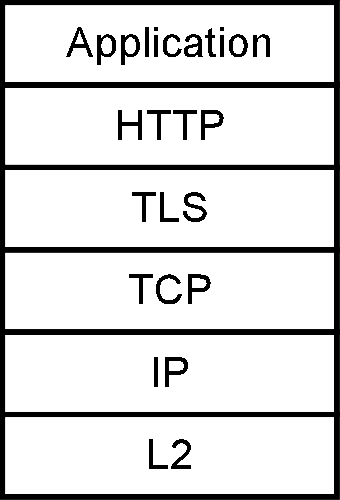
\includegraphics[width=0.25\textwidth]{5g-stack.pdf}
    \end{center}
    \caption{5G Control Plane Protocol Stack, according to TS 29.573 (\cite{3gpp.29.573}, 11)}
    \label{fig:5g-stack}
\end{wrapfigure}

\gls{3gpp} Release 15 features a redesigned protocol stack for signaling traffic between 5G core network functions, illustrated in figure \ref{fig:5g-stack}.
Rather than relying on specialized protocols that are almost exclusively used in previous generations of mobile networks, 5G makes broad use of protocols, formats, and principles popular in the web services domain.
The \gls{tcp} is used as a transport protocol, rather than \gls{sctp}.
On top of that, the \gls{ip} carries \gls{http} messages that may optionally be protected by \gls{tls}.
Inside the \gls{http} body additional information structured as \gls{json} objects can be transferred.
Communication between 5GC \glspl{nf} follows a client server model, with \glspl{api} that are modelled according to the constraints of \gls{rest}.
All signaling messages are completely self-contained, alleviating the need to store state information on server side across multiple requests and also allowing for the possibility of caching responses by clients and intermediaries.

\bigskip

The above-mentioned changes to the protocol stack also extend to the signaling channel between different \glspl{plmn}, i.e. the N32 interface.
But aside from modernizing the protocols, a redesigned Core Network architecture entails further changes to enhance interconnect security.
Whereas earlier mobile generations only specify protection on transport layer by means of IPsec, which in practice is rarely used due to operator requirements cited in the previous section, 5G aims to offer more flexible protection on application layer.
For this purpose, a dedicated Network Function is introduced to ensure security on the N32 interface.
The \gls{sepp} is tasked with applying confidentiality and integrity protection to outbound signaling messages, depending on an operator-controlled protection policy.
Simultaneously, it is the single point of contact for all inbound signaling traffic, ensuring mutual authentication with all peer \glspl{sepp}, enforcing message integrity, rate limits, and further security checks.
A complete list of \gls{sepp} requirements is given in TS 33.501 (\cite{3gpp.33.501}, 31)
When an \gls{nf} exchanges Control Plane messages with another \gls{nf} in a different \gls{plmn}, it sends these messages towards a \gls{sepp} in its own network.
The \gls{sepp} transforms the complete message into a \gls{json} object before applying security on the individual information elements contained.
Protection is provided by means of \gls{jwe} and symmetric keys shared between peer \glspl{sepp}, which is able to ensure integrity, confidentiality, or both.
Afterwards, the transformed message is sent towards the roaming partner's \gls{sepp} via one or more \gls{ipx} providers.
Certain \gls{ipx} provider may add changes to the transported messages, using the \gls{json} patch method (\cite{rfc6902}).
Patches are digitally signed using \gls{jws} and asymmetric cryptography.
The related public keys must be known to the involved \gls{plmn} operators.
Once a \gls{sepp} receives a incoming N32 message, it validates the integrity of the original contents and any patches added by \gls{ipx} providers.
If this first validation is successful and the \gls{ipx} patches only modify information elements that are allowed to be accessed, the \gls{sepp} transforms the \gls{json} element back into a separate signaling message, applying the suggested changes in the process.
The resulting signaling message is forwarded to the destination \gls{nf}.

\subsection{The PRINS Protocol}
\subsubsection{Protocol Structure}

The 5G inter-operator signaling protocol provides security for messages on the N32 interface between two \glspl{sepp}.
It allows these two endpoints to specify the level of protection prior to establishing a connection using so-called protection policies.
The protocol is comprised of two logical channels.
\\

\textbf{N32-c} is an end-to-end protected \gls{tls} connection used for session management.
Once an interconnect session is established, each of the communicating \glspl{sepp} sets up an N32-c channel to be able to send and receive such messages by its peer.
Messages exchanged via this channel serve the purpose of:

\begin{enumerate}[label=--]
    \item Session key agreement and refesh
    \item Session parameter agreement, e.g. protection policies and cryptographic profiles
    \item Error handling throughout the session
\end{enumerate}

In case two \glspl{plmn} are directly connected, without the need for any intermediaries, there is also the possibility of utilizing the N32-c channel to transfer signaling messages directly, without the use of \gls{prins}.
This purely \gls{tls} based option is highlighted for completeness sake and shall not be analyzed in details, for the reasons listed in section~\ref{sec:goal}.
\\

\textbf{N32-f} is a \gls{prins} protected connection carrying the actual inter-operator signaling messages.
The level of protection provided on this channel is determined by two types of protection policies, specified by each communicating party:

\begin{enumerate}[label=--]
    \item \textit{Data-type encryption policy}, specifying what types of information elements contained in signaling messages require confidentiality protection.
    \item \textit{Modification policy}, specifying what information elements are allowed to be modified by \gls{ipx} providers.
\end{enumerate}

The data-type encryption policy is supported by a \textit{\gls{nf} \gls{api} data-type placement mapping}, defining the data-type of a particular information element.
\gls{prins} expects this policy to be the same in both communicating \glspl{sepp} in order to rule out inconsistencies in the confidentiality requirements.
The modification policy defined by each communicating party is only applicable to the \gls{ipx} provider that the defining \gls{mno} has a business relationship with.

An N32-f session is identified by a \textit{N32-f context} -- supplementary information stored by each \gls{sepp} in order to correlate different messages.
This information can be summarized as follows:

\begin{enumerate}[label=--]
    \item \textit{N32-f context ID}, uniquely identifying messages belonging to a given session
    \item \textit{N32-f peer information}, containing the remote \gls{plmn} ID, remote \gls{sepp} ID, and its \gls{ip} address
    \item \textit{N32-f security context}, incl. agreed session keys and cipher suites, protection policies, session counters and initialization vectors, and an \gls{ipx} security information list
    \item \textit{N32-f context information}, containing session validity information and the decision to use \gls{prins} or \gls{tls}
\end{enumerate}


\begin{figure}[t]
    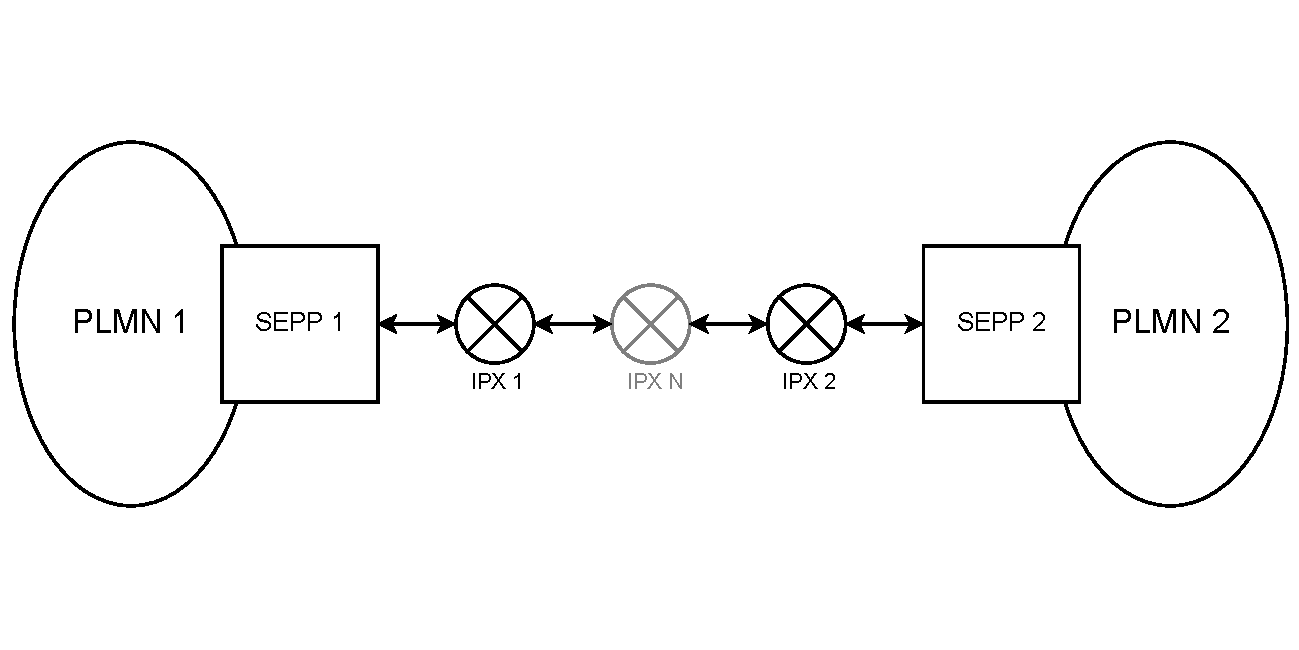
\includegraphics[width=\linewidth]{5g-roaming-arch.pdf}
    \centering
    \caption{5G interconnect architecture, according to TS 33.501 (\cite{3gpp.33.501}, 128)}
    \label{fig:n32}
\end{figure}


\subsubsection{N32-c Sequence}

\subsubsection{N32-f Sequence}

\subsubsection{Threat Model}
